% section2_2_prior.tex — Module B: Bo
% Addresses QHM Core Task 1, §3.2 (Prior).
\subsection{Prior Specification}\label{sec:prior}

Having established the Normal likelihood in Section~\ref{sec:likelihood}, completing the Bayesian model requires specifying prior distributions for the four unknown parameters: the regression coefficients $\beta_0,\, \beta_1,\, \beta_2$, and the residual standard deviation $\sigma$. Following the recommendation of the project handout, we adopt \emph{weakly informative} priors, defined here as priors broad enough to allow the likelihood to dominate over the moderate sample size $n = 360$, yet sufficiently restrictive to exclude values that would contradict basic physical understanding of bike-sharing demand. This choice both encodes our pre-data agnosticism about the magnitude and direction of each effect and creates the conditions under which the posterior is informed primarily by the data, allowing meaningful comparison with the frequentist baseline of Section~\ref{sec:frequentist}.

\subsubsection{Distributional Forms and Hyperparameters}

For the regression coefficients we adopt independent Normal priors centred at zero,
\begin{equation}
    \beta_j \;\sim\; \mathcal{N}\!\left(0,\; 10000^{2}\right), \qquad j = 0,\, 1,\, 2,
\end{equation}
each with prior mean, median, and mode coinciding at zero, prior standard deviation $10{,}000$, and an implied 95\% prior credible region of approximately $(-19{,}600,\; 19{,}600)$.

For the residual standard deviation we adopt a Half-Normal distribution to enforce the structural constraint $\sigma > 0$:
\begin{equation}
    \sigma \;\sim\; \text{Half-Normal}\!\left(\text{scale} = 3000\right).
\end{equation}
The Half-Normal distribution with scale parameter $s = 3000$ has prior median $s\,\Phi^{-1}(0.75) \approx 2024$, prior mean $s\sqrt{2/\pi} \approx 2394$, prior standard deviation $s\sqrt{1 - 2/\pi} \approx 1808$, and 95th percentile $s\sqrt{2}\operatorname{erf}^{-1}(0.95) \approx 5880$. Combining these priors with the likelihood from Section~\ref{sec:likelihood}, the complete generative model can be written
\begin{align}
    \beta_0,\, \beta_1,\, \beta_2 &\stackrel{\text{iid}}{\sim} \mathcal{N}(0,\, 10000^{2}), \\
    \sigma &\sim \text{Half-Normal}(3000), \\
    \mu_i &= \beta_0 + \beta_1\,\texttt{temp}_i + \beta_2\,\texttt{hum}_i, \\
    \texttt{cnt}_i \mid \mu_i,\, \sigma &\sim \mathcal{N}(\mu_i,\, \sigma^{2}), \quad i = 1, \dots, 360.
\end{align}

\begin{table}[htbp]
\centering
\caption{Prior distributions and the implied measures of location and dispersion. For the Half-Normal prior the moments are derived from its scale parameter as detailed in the text.}
\label{tab:priors}
\begin{tabular}{lllcc}
\hline
Parameter & Distribution & Hyperparameters & Prior mean & Prior SD \\
\hline
$\beta_0$ & Normal      & $\mu = 0,\; \sigma = 10000$ & $0$            & $10000$ \\
$\beta_1$ & Normal      & $\mu = 0,\; \sigma = 10000$ & $0$            & $10000$ \\
$\beta_2$ & Normal      & $\mu = 0,\; \sigma = 10000$ & $0$            & $10000$ \\
$\sigma$  & Half-Normal & scale $= 3000$              & $\approx 2394$ & $\approx 1808$ \\
\hline
\end{tabular}
\end{table}

\subsubsection{Justification of Hyperparameter Choices}

The exploratory analysis of Module~A establishes that the response \texttt{cnt} ranges from $22$ to $8555$, with sample mean $4392$ and sample standard deviation $1936$, while the predictors \texttt{temp} and \texttt{hum} are min--max normalised to the unit interval $[0, 1]$. Plausible regression coefficients are therefore on the order of $10^{3}$, since the largest credible change in expected \texttt{cnt} attributable to a single normalised covariate cannot greatly exceed the empirical range of \texttt{cnt} itself. Setting the prior standard deviation of each $\beta_j$ to $10{,}000$ ensures that approximately 95\% of the prior mass lies within $(-19{,}600,\, 19{,}600)$, comfortably enveloping the OLS point estimates of Section~\ref{sec:frequentist} ($\hat\beta_0 \approx 2548,\, \hat\beta_1 \approx 6796,\, \hat\beta_2 \approx -2370$) and excluding only values so extreme that they would imply effects substantially exceeding the entire range of the response. Centring the priors at zero is consistent with our pre-data agnosticism about both the sign and the magnitude of each weather effect.

The Half-Normal scale of $3000$ for $\sigma$ was selected so that its prior median ($\approx 2024$) is comparable in order of magnitude to the empirical standard deviation of \texttt{cnt} ($\approx 1936$), with sufficient mass at smaller values to accommodate the OLS residual standard error reported by Module~A ($\hat\sigma_{\mathrm{OLS}} = 1497$), while values larger than approximately $10{,}000$ — which would imply implausibly diffuse residuals on the scale of the data — are effectively excluded. The choice of a Half-Normal rather than, say, an Inverse-Gamma reflects current best practice for variance-scale priors in modern Bayesian workflows: it places its highest density at modest values of $\sigma$ without imposing the sharp-tailed pathologies of Inverse-Gamma priors at small scales.

We emphasise that the prior standard deviations selected here are deliberately several times larger in magnitude than the eventual posterior standard deviations reported in Section~\ref{sec:posterior}. This bandwidth ensures that the posterior is dominated by the likelihood rather than by the prior, satisfying the handout's stated philosophy that a weakly informative prior should rule out clearly implausible values without strongly favouring any particular value, and creating an appropriate baseline against which Module~C may assess sensitivity to alternative prior specifications in Section~\ref{sec:sensitivity}.

\subsubsection{Prior Predictive Check}

To verify that the chosen priors are reasonable on the natural scale of the response, we drew $500$ samples from the prior predictive distribution of \texttt{cnt} --- the marginal distribution of simulated observations obtained by drawing parameters from the prior and then drawing \texttt{cnt} values from the corresponding sampling distribution. The resulting empirical distribution is shown in Figure~\ref{fig:prior_pred}.

\begin{figure}[htbp]
    \centering
    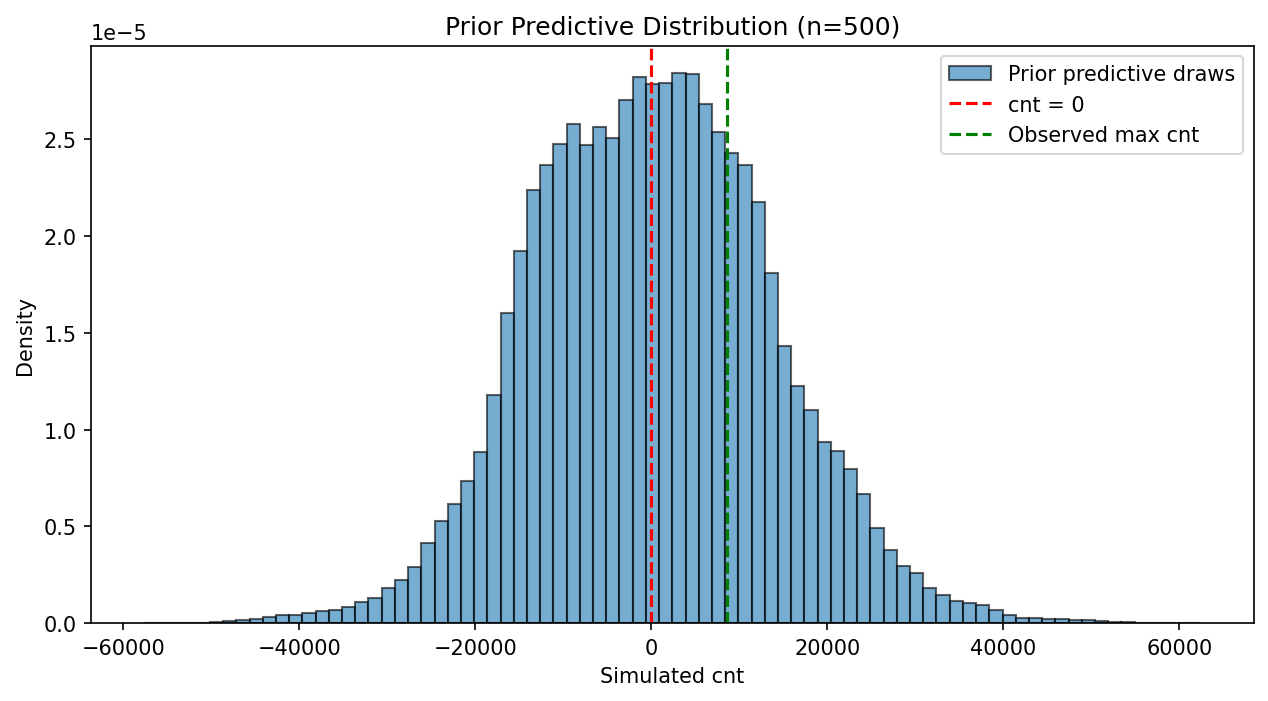
\includegraphics[width=0.7\textwidth]{../results/figures/prior_predictive.png}
    \caption{Prior predictive distribution of \texttt{cnt} based on $500$ draws from the joint prior. The dashed lines mark $\texttt{cnt} = 0$ and the maximum observed value $8555$. The prior assigns substantial mass to values between $-30{,}000$ and $30{,}000$, far exceeding the observed range and confirming the weakly informative character of the specification.}
    \label{fig:prior_pred}
\end{figure}

The prior predictive distribution is approximately symmetric about zero, with the bulk of probability mass spanning roughly $\pm 30{,}000$ --- about seven times the empirical range of \texttt{cnt}. This wide coverage confirms that the prior does not pre-determine the location, scale, or sign of the response. As is typical for weakly informative formulations on regression coefficients, the prior assigns positive density to negative \texttt{cnt} values, which are physically impossible; this is an acceptable limitation of unconstrained Normal priors on coefficients, since the likelihood will appropriately constrain the posterior to the realistic positive range once the data are observed, as confirmed by the posterior summaries of Section~\ref{sec:posterior}.
